% IEEE IV 2027 submission draft (double-blind, 6 pages incl. references, +2 paid).
% Before submitting: remove the red \draftnote blocks, check anonymity, keep the IEEE
% copyright notice OFF.  Source style: one paragraph per line.
\documentclass[conference]{IEEEtran}

\usepackage{iftex}
\ifXeTeX
  \usepackage{fontspec}
  \setmainfont{texgyretermes}[Extension=.otf, UprightFont=*-regular, BoldFont=*-bold, ItalicFont=*-italic, BoldItalicFont=*-bolditalic]
\fi
\usepackage{graphicx}
\usepackage{amsmath}
\usepackage{amssymb}
\usepackage{booktabs}
\usepackage{xcolor}
\usepackage{url}
\usepackage[hidelinks]{hyperref}
\usepackage[capitalize]{cleveref}

\newcommand{\st}[1]{\textsc{#1}}
\newcommand{\draftnote}[1]{\textcolor{red}{#1}}

\title{Response Bias, Not Perception, Breaks Temporal State Estimation\\from Foundation-Model Evidence under Domain Shift}
\author{\IEEEauthorblockN{Anonymous Authors}\IEEEauthorblockA{Paper under double-blind review}}

\begin{document}
\maketitle

\draftnote{\textbf{Draft status.} The California four-state labels (\cref{sec:benchmark}) are a first pass pending human verification. Every number in \cref{sec:ood,sec:adapt} is regenerated from the verified labels by \texttt{pipeline/california\_4state.py}, \texttt{california\_adapt.py} and \texttt{annotation/draft\_eval.py}; do not cite them before that run.}

\begin{abstract}
Driving systems increasingly turn the per-frame answers of a foundation model into a temporal state: a detector or a vision--language model says what is in the frame, and a filter or segmenter decides when a situation starts and ends. We study this split on work-zone traversal, where the state is one of \st{outside}, \st{approaching}, \st{inside} and \st{exiting}, with every system running on an embedded GPU. In domain, six temporal layers built on a detector and a 4B world model reach macro-F1 0.46 to 0.55, and the best of them resolves the usual trade-off between boundary quality and false alarms. We then introduce a four-state benchmark from 51 minutes of California driving at day, dusk, night, rain and fog, labeled separately for whether work is visible and whether it concerns the ego vehicle. Three results follow. First, the metric commonly used for out-of-domain evidence, a hit anywhere in a short window, is dominated by response bias: the world model answers ``yes'' on 40\% of seconds with no work in view, so 72\% of work-free 7-second windows already count as hits. Second, once bias is removed, perception transfers unevenly rather than failing: the detector separates work from no work better by day (AUC 0.80 against 0.67), the world model better at night and in weather (0.70--0.77 against 0.52--0.62), and neither can tell relevant from irrelevant work (AUC below 0.5 for both). Third, the in-domain ranking of temporal layers inverts: the best in-domain estimator falls from 0.546 to 0.295 macro-F1 and from 26 to 68 false alarms per hour. Unsupervised re-estimation of the estimator's emission model does not repair this, because without labels a shift in how often a model says ``yes'' is indistinguishable from a shift in how often work is present. We argue that temporal layers over foundation-model evidence should be evaluated, and adapted, against response bias rather than against perception.
\end{abstract}

\section{Introduction}
\label{sec:intro}

A common way to put a foundation model in a vehicle is to ask it about each frame and let a small temporal model do the rest. A detector counts cones; a vision--language model (VLM) answers ``are there road-work indicators in this scene?''; a Bayesian filter, a vote, or a temporal convolutional network turns those answers into a state that an advisory can act on. The split is attractive because the expensive part is general and pretrained, and the cheap part is specific and easy to fit.

This paper asks what happens to that split under domain shift. Our running example is work-zone traversal, a four-state problem (\st{outside}, \st{approaching}, \st{inside}, \st{exiting}) where the boundaries matter most and where errors in both directions are costly~\cite{nhtsa2023,priorsystem2026}. Every system we study runs on a Jetson AGX Orin, under a replay protocol in which each system's own latency decides which frames it sees.

In domain, the temporal layer is where the gains are. On 208 held-out ROADWork videos~\cite{ghosh2025roadwork}, replacing a detector's hand-set smoothing constants with a filter whose parameters are counted from data raises macro-F1 from 0.470 to 0.536 on the same detector evidence, and adding a world model's answers gives 0.546 at 25.9 false alarms per hour. A learned causal segmenter ties that macro-F1. Read in isolation, these results say that better temporal modeling is the path forward.

Out of domain the picture changes, and the reason is not the one we expected. Our earlier measurements used the usual out-of-domain proxy, a hit anywhere in a short window after an annotated event, and reported the world model finding 95\% of California work-zone signs against 72\% for the detector. That number is mostly response bias. The world model says ``yes'' on 40\% of work-free seconds, so a 7-second window with no work in view already scores a hit 72\% of the time. To measure transfer properly we labeled every second of the footage twice: whether work is visible, and whether it concerns the ego vehicle.

With those labels, perception does not so much fail as move. By day the detector separates work from no work better; at night and in weather the world model does. Neither separates relevant from irrelevant work at all. The temporal layers, fitted to in-domain response rates, then turn each model's new bias into errors: the best in-domain estimator becomes one of the worst, with false alarms more than doubling. Re-estimating the estimator's emission model on unlabeled target data does not help, and we show why: the shift in how often a model says ``yes'' and the shift in how often work is present are not identifiable from the evidence alone.

Our contributions are:
\begin{enumerate}
\item A four-state work-zone benchmark from 51 minutes of California driving across day, dusk, night, rain and fog, labeled per second for work visibility and ego-relevance, with the labeling guideline and tools.
\item An evaluation that separates perception (bias-free discrimination), ego-relevance, and temporal action, and shows that window-hit metrics for out-of-domain evidence are dominated by response bias.
\item A controlled comparison of six temporal layers over the same detector and world-model evidence, in domain and out of domain, showing that the in-domain ranking inverts.
\item A negative result for unsupervised emission re-estimation, with an identifiability argument for why it fails.
\end{enumerate}

\section{Related Work}
\label{sec:related}

\paragraph{Work zones.} ROADWork~\cite{ghosh2025roadwork} provides work-zone images, videos and descriptions from 18 U.S. cities and shows large gains from in-domain fine-tuning. The four-state traversal task and the detector pipeline we use as a baseline come from \cite{priorsystem2026}, which pairs a ROADWork-trained detector with CLIP verification~\cite{radford2021clip}, exponential smoothing and hysteresis. Earlier systems used structured environment models~\cite{shi2021workzone} or frame classification~\cite{abodo2018shrp}.

\paragraph{Foundation models as driving sensors.} VLMs are used for planning~\cite{hwang2024emma,tian2024drivevlm}, description~\cite{marcu2024lingoqa} and physical reasoning~\cite{nvidia2025cosmosreason,nvidia2026cosmos3,alpamayo2026}, and quantization~\cite{lin2024awq} with embedded runtimes~\cite{trtedgellm} brings small ones to automotive hardware. Most evaluations score the model's answers; we score the state a system builds from them.

\paragraph{Temporal segmentation.} Assigning a state to every frame is temporal action segmentation, for which MS-TCN~\cite{farha2019mstcn} introduced multi-stage dilated convolutions and a smoothing loss. We train a strictly causal variant with modality dropout~\cite{neverova2016moddrop}.

\paragraph{Shift and test-time adaptation.} Label-shift methods re-estimate class priors from unlabeled target data under the assumption that class-conditional distributions are fixed~\cite{saerens2002adjusting,lipton2018bbse}; test-time adaptation updates model parameters from unlabeled target inputs~\cite{wang2021tent}. Our setting violates the label-shift assumption in the specific way that makes it hard: what moves is the conditional response of the sensor, and it moves together with the prior.

\section{Systems and In-Domain Results}
\label{sec:systems}

\paragraph{Evidence.} Two models produce evidence on the same Orin. The detector is a ROADWork-trained YOLO whose per-frame score weights detected cues by category~\cite{priorsystem2026}; it runs at about 22\,Hz. The world model is Cosmos3-Edge~\cite{nvidia2026cosmos3}, a 4B physical-AI model whose reasoner we quantize to INT4 (W4A16 AWQ) and run with TensorRT; it has never seen work-zone training data. It answers three fixed prompts: a binary existence \st{gate}, a sign transcription matched against a keyword list (\st{sign}), and a structured description matched against an object lexicon (\st{desc}). One pass of the three takes about 1.5\,s.

\paragraph{Temporal layers.} All six layers consume the same evidence.
\emph{Cascade}: the world model's evidence-first state machine with votes over a short window, calibrated for this model ($N{=}3$, $K_\text{enter}{=}3$, $K_\text{exit}{=}2$, $K_\text{fade}{=}1$).
\emph{Detector, counted filter}: a forward filter over the four states whose emission $P(\text{observation}\mid\text{state})$ and per-second transition rates are counted on 312 calibration videos, observing the detector score only.
\emph{Joint}: the same filter over a joint observation of detector score (six buckets), world-model evidence (six levels) and answer age (three buckets), 108 cells, fitted on 100 or on all 312 calibration videos.
\emph{Joint, no detector}: the joint filter refitted without the detector stream.
\emph{TCN}: a causal three-stage MS-TCN (100{,}780 parameters) trained on the same calibration evidence with modality dropout and early stopping.
The filters scale the log-likelihood by $dt/\tau$ with $\tau{=}0.5$\,s so that near-duplicate frames do not count as independent evidence.

\paragraph{In-domain protocol.} We use the 520-video ROADWork traversal benchmark of \cite{priorsystem2026}, split by video into 312 calibration and 208 validation videos (1.78\,h). All fitting and selection use calibration; we report validation. Replay is latency-honest: after each measured cycle the video advances by that cycle's duration and skipped frames are never seen. Metrics follow \cite{priorsystem2026}; false alarms per hour count predicted active intervals that overlap no annotated active interval.

\begin{table}[t]
\centering
\caption{In domain: 208 ROADWork validation videos, same evidence, same device. FA/h: false alarms per hour.}
\label{tab:indomain}
\footnotesize
\setlength{\tabcolsep}{4pt}
\begin{tabular}{@{}lcccc@{}}
\toprule
Temporal layer & Macro F1 & IoU \st{appr} & IoU \st{exit} & FA/h \\
\midrule
Detector, hand-set (\cite{priorsystem2026}, our port) & 0.470 & 0.124 & 0.106 & 30.9 \\
Cascade (world model) & 0.515 & \textbf{0.278} & 0.071 & 64.6 \\
Detector, counted filter & 0.536 & 0.233 & 0.148 & \textbf{18.5} \\
Joint (100) & \textbf{0.550} & 0.262 & 0.163 & 33.2 \\
Joint (312) & 0.546 & 0.246 & 0.160 & 25.9 \\
Joint, no detector & 0.460 & 0.211 & 0.017 & 42.7 \\
Causal TCN & \textbf{0.550} & 0.260 & \textbf{0.169} & 71.9 \\
\bottomrule
\end{tabular}
\end{table}

\Cref{tab:indomain} is the in-domain picture. Counting the filter's parameters instead of setting them by hand is worth 0.066 macro-F1 on the detector's own evidence; adding the world model is worth another 0.010. The joint estimator fitted on all calibration videos is the only layer above the hand-set detector at a lower false-alarm rate, and the TCN ties the best macro-F1 at nearly three times its alarms. The same filter without the detector loses \st{exiting} almost entirely, because the fading detector score is what signals that a zone is ending. In-domain paired bootstrap intervals (10{,}000 video-level replications) put the joint estimator above the detector by $+0.076$ macro-F1 ($[+0.047, +0.105]$) with no significant difference in false alarms.

\section{A Four-State Out-of-Domain Benchmark}
\label{sec:benchmark}

\paragraph{Footage.} Fourteen dashcam recordings from Merced, Fresno and highways CA-50 and CA-99 in California, 51.0 minutes in total, with a different camera from ROADWork and conditions ROADWork does not contain: day (19.0\,min), evening (1.8), sunset (5.3), night (10.0), night with rain (9.0) and night with fog (6.0). The recordings were made to capture work zones, so work is visible in about half of the footage.

\paragraph{Labels.} Every second receives two labels (guideline in the supplement). \emph{Visible}: any temporary traffic-control element or active work is in view. \emph{Ego-relevant}: the work regulates or affects the ego vehicle's direction of travel, which is the condition under which the four states are defined, as in \cite{priorsystem2026}. The four states then follow the source benchmark's conventions. Keeping the two labels separate lets us ask whether a model sees work at all and, separately, whether it can tell work that matters from work that does not, such as cones on the opposite carriageway or equipment in a parking lot. Of 3{,}064 labeled seconds, 1{,}484 show no work, 160 show work that does not concern the ego vehicle, and 1{,}420 are ego-relevant. \draftnote{Labels are a first pass made from contact sheets at one frame every two seconds and are being verified by a person at full frame rate with a keyboard tool; stretches the first pass marked as low confidence are listed for the verifier.}

\paragraph{Evidence record.} We record every evidence channel of both models once, at 1\,Hz over the whole footage, and evaluate all temporal layers by replaying that record. The record reproduces our earlier live window measurements exactly for the five systems we had run on GPU. Layers that run faster live are approximated: filters step once per second with a fresh world-model answer, and the TCN sees each second's features held over its 10\,Hz grid.

\section{What Transfers}
\label{sec:ood}

\subsection{Window hits measure response bias}

\begin{figure}[t]
\centering
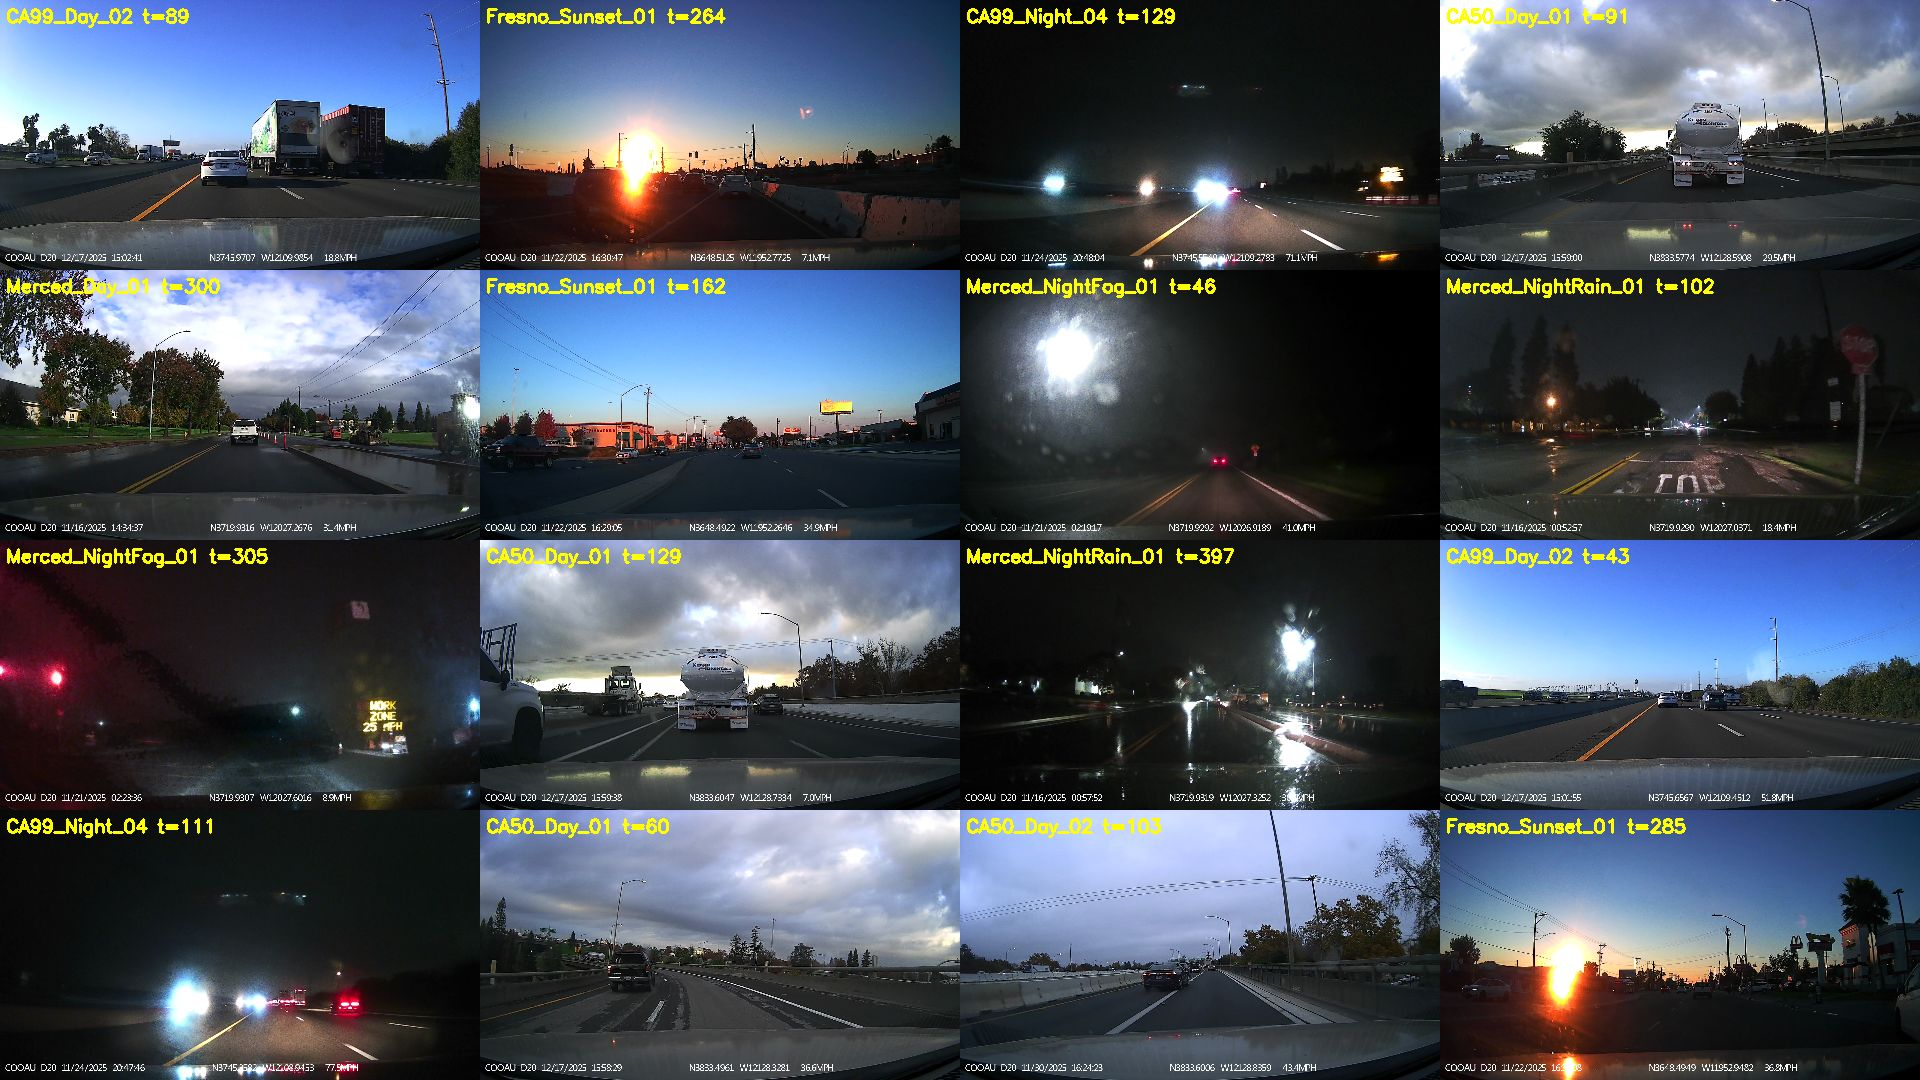
\includegraphics[width=\linewidth]{fig_falseyes.jpg}
\caption{Sixteen random California frames on which the world model's gate answers ``yes'' at least 20\,s away from any annotated sign. Most show no work zone.}
\label{fig:falseyes}
\end{figure}

The common proxy for out-of-domain evidence counts an event as detected if a model responds anywhere in a short window after it. On the 39 annotated sign approaches in this footage, that proxy gives the world model 95\% and the detector 72\%. The same rule applied to 7-second windows in which no work is visible gives 72\% and 18\%. The world model answers ``yes'' on 40.2\% of work-free seconds, the detector responds on 5.6\%. The window proxy is therefore mostly a measurement of how often a model says ``yes'', and \cref{fig:falseyes} shows what those answers look like.

\subsection{Perception moves; ego-relevance never arrives}

\begin{table}[t]
\centering
\caption{Per-second discrimination on California (AUC; 0.5 is chance). Perception: visible work against no work. Ego-relevance: relevant against visible-but-irrelevant work.}
\label{tab:auc}
\footnotesize
\setlength{\tabcolsep}{4pt}
\begin{tabular}{@{}lccc@{}}
\toprule
 & seconds (pos / neg) & World model & Detector \\
\midrule
Perception, all & 1176 / 1484 & 0.72 & 0.72 \\
\quad day & 590 / 462 & 0.67 & \textbf{0.80} \\
\quad sunset & 142 / 158 & 0.59 & \textbf{0.81} \\
\quad night & 118 / 374 & \textbf{0.70} & 0.52 \\
\quad night, rain & 156 / 284 & \textbf{0.77} & 0.62 \\
\quad night, fog & 158 / 160 & \textbf{0.76} & 0.60 \\
Ego-relevance & 1420 / 160 & 0.47 & 0.43 \\
\bottomrule
\end{tabular}
\end{table}

AUC removes the response rate and asks only whether a model responds more when work is there. \Cref{tab:auc} shows that neither model fails outright and neither dominates. The detector is the better perceiver in daylight and at sunset. At night, in rain and in fog, the world model is better, which matches the earlier window result in direction but at a fraction of its size. On ego-relevance both are below chance: they respond to irrelevant work at least as often as to relevant work. This extends to a new domain the failure we observed in domain, where the residual false positives of every VLM system were correctly described objects that did not concern the vehicle.

\subsection{The in-domain ranking inverts}

\begin{table}[t]
\centering
\caption{Four-state results on California, same six temporal layers as \cref{tab:indomain}, replayed on the 1\,Hz evidence record. \draftnote{Draft labels.}}
\label{tab:ood}
\footnotesize
\setlength{\tabcolsep}{3.2pt}
\begin{tabular}{@{}lcccccc@{}}
\toprule
Temporal layer & Acc. & F1 & IoU \st{ap} & IoU \st{in} & \st{in} rec. & FA/h \\
\midrule
Cascade & 55.0 & 0.388 & 0.156 & 0.338 & 75.0 & 56.5 \\
Detector, counted & 57.5 & 0.296 & 0.028 & 0.221 & 31.2 & \textbf{14.1} \\
Joint (100) & 48.4 & 0.304 & 0.044 & 0.234 & 62.5 & 64.7 \\
Joint (312) & 47.8 & 0.295 & 0.035 & 0.222 & 37.5 & 68.2 \\
Joint, no detector & \textbf{57.7} & \textbf{0.414} & \textbf{0.231} & \textbf{0.395} & 81.2 & 90.6 \\
Causal TCN & 53.7 & 0.336 & 0.045 & 0.312 & \textbf{87.5} & 60.0 \\
\bottomrule
\end{tabular}
\end{table}

\Cref{tab:ood} replays the six layers on California. Five of the six layers lose between 0.13 and 0.25 macro-F1; the world-model-only filter loses 0.05. The order changes. The joint estimator, best in domain inside the alarm budget, falls to 0.295 macro-F1 with 68 false alarms per hour, and by day it produces 117 per hour. The detector-only filter keeps a low alarm rate but recovers only 31\% of \st{inside} events, because at night the detector is nearly silent. The best macro-F1 comes from the world model alone, through the joint filter without its detector stream or through the cascade, and at 57 to 91 false alarms per hour.

The two per-model biases of \cref{sec:ood} explain most of this. A filter counted in domain has learned how often each model responds in each state. Out of domain the world model responds more everywhere and the detector less at night, and a filter that trusts in-domain response rates reads the first as work that is not there and the second as the absence of work that is. The joint table is hit twice: its most informative in-domain cells are the ones where the two models agree, and out of domain they rarely agree for the right reason.

\section{Adapting Without Labels}
\label{sec:adapt}

Because the transition structure of a work zone is a property of roads rather than of sensors, a natural fix keeps the counted transition rates and re-estimates only the emission table from unlabeled target evidence. We run expectation--maximization with forward--backward posteriors under the same tempered likelihood the filter uses, and a Dirichlet prior centred on the in-domain table:
\[
e'_{s,o} \;\propto\; \lambda N \pi_s\, e^\text{src}_{s,o} + \textstyle\sum_t \gamma_t(s)\,[o_t = o],
\]
where $N$ is the number of target observations, $\pi$ the in-domain state prior, and $\lambda$ the weight of the source table. We fix $\lambda{=}0.5$ in advance and report $0.25$ and $1.0$ as sensitivity. We adapt either on all target videos (transductive) or, more strictly, on the other thirteen videos only.

\begin{table}[t]
\centering
\caption{Unsupervised emission adaptation on California (leave-one-video-out). \draftnote{Draft labels.}}
\label{tab:adapt}
\footnotesize
\setlength{\tabcolsep}{4pt}
\begin{tabular}{@{}llccc@{}}
\toprule
Filter & Emission & F1 & IoU \st{in} & FA/h \\
\midrule
Joint (312) & source & 0.295 & 0.222 & 68.2 \\
 & adapted, $\lambda{=}0.25$ & 0.330 & 0.269 & 90.6 \\
 & adapted, $\lambda{=}0.5$ & 0.324 & 0.264 & 83.5 \\
 & adapted, $\lambda{=}1.0$ & 0.312 & 0.246 & 87.0 \\
\midrule
Joint, no detector & source & 0.414 & 0.395 & 90.6 \\
 & adapted, $\lambda{=}0.5$ & 0.410 & 0.396 & 187.0 \\
\bottomrule
\end{tabular}
\end{table}

\Cref{tab:adapt} shows that adaptation buys at most 0.035 macro-F1 and always raises false alarms, doubling them for the world-model-only filter; transductive adaptation gives the same pattern. The failure is structural. The observation likelihood of an HMM and its state occupancy trade off against each other: more ``yes'' answers can be explained by a sensor that says ``yes'' more often in the same states, or by more time spent in active states. The source table and the transition prior break the tie in domain. Out of domain the evidence alone does not, and EM takes the explanation that the prior makes cheapest, which is more work. This is the label-shift problem~\cite{saerens2002adjusting,lipton2018bbse} with its key assumption removed: the class-conditional response is exactly what moved.

The practical reading is that adaptation needs a signal about the sensor that does not pass through the state. Two such signals are available without labels in principle: responses on inputs known to be negative, such as frames from a stretch the vehicle has already classified with high confidence, and agreement structure between sensors whose biases move differently, which \cref{tab:auc} shows is the case here. We leave both to future work; the benchmark is designed to evaluate them.

\section{Limitations}
\label{sec:limits}

\draftnote{The California labels are a first pass awaiting human verification, and all out-of-domain numbers depend on them.} The benchmark is 51 minutes from one region and one camera, with fewer than ten minutes in each weather condition, so per-condition values are descriptive. Out-of-domain results are replayed at 1\,Hz, which approximates layers that run faster live. We study one detector and one world model; whether other VLMs show the same response bias is untested. The in-domain split shares drives between calibration and validation, and fine-tuning data for the detector and the benchmark both derive from ROADWork.

\section{Conclusion}
\label{sec:conclusion}

When a temporal model sits on top of a foundation model's per-frame answers, in-domain evaluation measures the pair. Out of domain, the pair separates: perception shifts unevenly across conditions and sensors, ego-relevance is absent for every model we tried, and the temporal layer, fitted to in-domain response rates, turns the sensor's new bias into errors. The in-domain ranking of temporal layers is not informative about this, window-hit metrics hide it, and unsupervised re-estimation cannot undo it because bias and base rate are confounded. We release the benchmark, the labeling guideline and tools, the evidence record, and the replay harness so that temporal layers can be evaluated against response bias directly.

{\small
\bibliographystyle{IEEEtran}
\bibliography{references}
}

\end{document}
